\documentclass[10pt,a4paper]{amsart}
\usepackage[margin=19mm]{geometry}
\usepackage{amsmath,amssymb,mathtools}
\usepackage[scr=rsfs,cal=euler]{mathalfa}
\usepackage{xfrac}
\usepackage[unicode,hidelinks,bookmarks=false]{hyperref}
\newcommand{\ie}{i.e.\ }
\newcommand{\cf}{cf.\ }
\newcommand{\resp}{respectively\ }
\newcommand{\Subsection}{\subsection}
\providecommand{\nobreakdash}{\nobreak\hbox{-}}
\setlength{\emergencystretch}{2em}
\multlinegap0pt
\usepackage{tikz}
\usepackage{amssymb}
\usepackage{bm}
\usepackage{xcolor}
\usepackage{mathtools}
\usepackage[normalem]{ulem}
\usepackage{mdframed}
\usepackage{enumerate}
\newtheorem{lem}{Lemma}
\title{The Hom-Ext quiver and applications to exceptional collections}
\author{Kiyoshi Igusa, Ray Maresca}
\date{Source: arXiv:2509.16388v2 (CC BY 4.0)}
\begin{document}
\maketitle

\noindent\emph{Source and licence.} The Hom-Ext quiver and applications to exceptional collections. Version arXiv:2509.16388v2 (CC BY 4.0), distributed by arXiv under the Creative Commons Attribution 4.0 International licence, http://creativecommons.org/licenses/by/4.0/, as recorded in the arXiv licence metadata for this exact version and shown on the abstract page https://arxiv.org/abs/2509.16388v2. Full licence notice: \texttt{licenses/arxiv-2509.16388-CC-BY-4.0.txt}.\par\smallskip

\noindent\textit{Editorial scope.} Counted unit: the article's lem simple (source0.tex lines 2032--2034). The article's complete original proof of it is delivered with it (source0.tex lines 2036--2147, one \texttt{proof} environment of 112 lines). No mathematics is written, repaired or re-derived: the statement and the proof are the article's own lines, in the article's own notation, and no retained line is substituted or re-flowed.  No further source-local context is needed: every cross-reference of every retained line resolves inside the two delivered spans.  Nothing was omitted from any retained span, so the package carries no omission record.  No retained line contains a citation, so the wrapper carries no bibliography and no bibliography entry.  The retained lines contain the article's own diagram code, which the wrapper typesets with the standard tikz packages; no image file is delivered and the package declares no asset dependency.  Editorial formatting only, in addition: an AMS \texttt{amsart} preamble that restates the article's own declarations and macros used by the retained lines, namely the environments \texttt{lem} on separate counters, together with the standard packages those lines need.  The retained environments print in this document as Lemma 1 in order of appearance, whereas the article prints the same items with the numbering of its own full document.  The complete native source of the article as distributed in the arXiv e-print for this exact version is bundled unchanged as \texttt{sources/185372/source0.tex}.
\begin{lem}\label{lem: iso sends simple to simple}
    Let $\varphi:(Q^{\chi_1},R_1) \rightarrow (Q^{\chi_2},R_2)$ be an isomorphism of Hom-Ext quivers where $\chi_1$ and $\chi_2$ are two exceptional collections of a quiver of type $\tilde{\mathbb{A}}_{n-1}$. If $X_i \in \chi_1$ is a quasi-simple module, so is $\varphi(X_i)$.
\end{lem}

\begin{proof}
    Suppose that $\varphi$ is an isomorphism of Hom-Ext quivers, $X_i\in \chi_1$ is a quasi-simple left regular module, and for contradiction, that $\varphi(X_i)$ is not quasi-simple. The proof when $X_i$ is right-regular is analogous. Since $\chi_2$ is complete, there exists a left regular module $\varphi(X_{i_1})$ such that there is a surjection $\varphi(X_i) \rightarrow \varphi(X_{i_1})$, or an injection $\varphi(X_{i_1}) \rightarrow \varphi(X_i)$. We will assume the later case, as the proof in the former case is analogous. Again, by completeness of $\chi_2$, there is a chain of morphisms $\varphi(X_{i_k}) \leftrightarrow \cdots \leftrightarrow \varphi(X_{i_2}) \leftrightarrow \varphi(X_{i_1}) \rightarrow \varphi(X_i)$ in $(Q^{\chi_2},R_2)$ where $\varphi(X_{i_k})$ is a quasi-simple module and the two headed arrows indicate that the morphism can go either left or right. Since $\varphi$ is an isomorphism of Hom-Ext quivers, we have an analogous chain $X_{i_k} \leftrightarrow \cdots \leftrightarrow X_{i_2} \leftrightarrow X_{i_1} \rightarrow X_i$  in $(Q^{\chi_1},R_1)$ as in the following diagram.

\begin{center}


\tikzset{every picture/.style={line width=0.75pt}} %set default line width to 0.75pt        

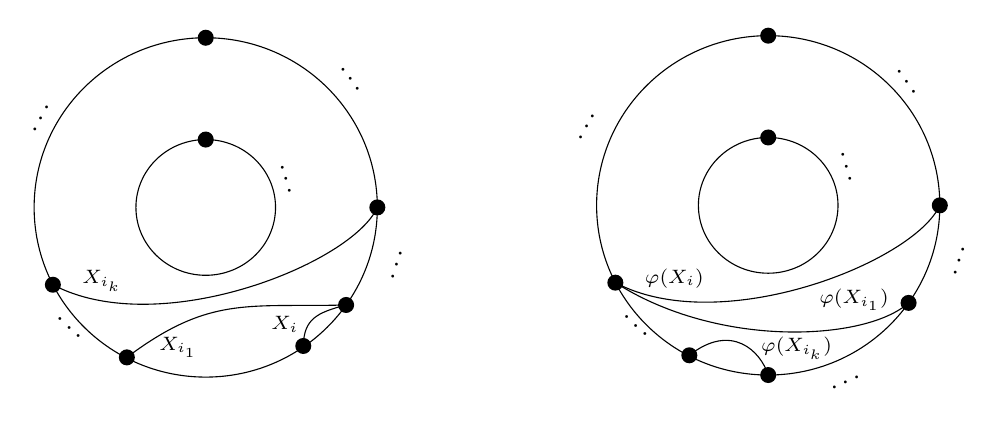
\begin{tikzpicture}[x=0.75pt,y=0.75pt,yscale=-1,xscale=1]
%uncomment if require: \path (0,213); %set diagram left start at 0, and has height of 213

%Shape: Donut [id:dp1666938723489756] 
\draw   (87.01,100.25) .. controls (87.01,82.19) and (102.06,67.55) .. (120.64,67.55) .. controls (139.21,67.55) and (154.27,82.19) .. (154.27,100.25) .. controls (154.27,118.31) and (139.21,132.95) .. (120.64,132.95) .. controls (102.06,132.95) and (87.01,118.31) .. (87.01,100.25)(37.96,100.25) .. controls (37.96,55.1) and (74.97,18.5) .. (120.64,18.5) .. controls (166.3,18.5) and (203.32,55.1) .. (203.32,100.25) .. controls (203.32,145.4) and (166.3,182) .. (120.64,182) .. controls (74.97,182) and (37.96,145.4) .. (37.96,100.25) ;
%Straight Lines [id:da4716612363540913] 
\draw    (167.64,167) ;
\draw [shift={(167.64,167)}, rotate = 0] [color={rgb, 255:red, 0; green, 0; blue, 0 }  ][fill={rgb, 255:red, 0; green, 0; blue, 0 }  ][line width=0.75]      (0, 0) circle [x radius= 3.35, y radius= 3.35]   ;
%Straight Lines [id:da030000684193490335] 
\draw    (188.27,147.25) ;
\draw [shift={(188.27,147.25)}, rotate = 0] [color={rgb, 255:red, 0; green, 0; blue, 0 }  ][fill={rgb, 255:red, 0; green, 0; blue, 0 }  ][line width=0.75]      (0, 0) circle [x radius= 3.35, y radius= 3.35]   ;
%Straight Lines [id:da7209275234162486] 
\draw    (203.32,100.25) ;
\draw [shift={(203.32,100.25)}, rotate = 0] [color={rgb, 255:red, 0; green, 0; blue, 0 }  ][fill={rgb, 255:red, 0; green, 0; blue, 0 }  ][line width=0.75]      (0, 0) circle [x radius= 3.35, y radius= 3.35]   ;
%Straight Lines [id:da6643909377532963] 
\draw    (82.64,172.5) ;
\draw [shift={(82.64,172.5)}, rotate = 0] [color={rgb, 255:red, 0; green, 0; blue, 0 }  ][fill={rgb, 255:red, 0; green, 0; blue, 0 }  ][line width=0.75]      (0, 0) circle [x radius= 3.35, y radius= 3.35]   ;
%Curve Lines [id:da5409909354917227] 
\draw    (167.64,167) .. controls (168,154) and (174,151) .. (188.27,147.25) ;
%Straight Lines [id:da5672065453552719] 
\draw    (120.64,18.5) ;
\draw [shift={(120.64,18.5)}, rotate = 0] [color={rgb, 255:red, 0; green, 0; blue, 0 }  ][fill={rgb, 255:red, 0; green, 0; blue, 0 }  ][line width=0.75]      (0, 0) circle [x radius= 3.35, y radius= 3.35]   ;
%Curve Lines [id:da2907493304000154] 
\draw    (82.64,172.5) .. controls (122.64,142.5) and (141,148.5) .. (188.27,147.25) ;
%Straight Lines [id:da7435227832526792] 
\draw    (47,137.5) ;
\draw [shift={(47,137.5)}, rotate = 0] [color={rgb, 255:red, 0; green, 0; blue, 0 }  ][fill={rgb, 255:red, 0; green, 0; blue, 0 }  ][line width=0.75]      (0, 0) circle [x radius= 3.35, y radius= 3.35]   ;
%Curve Lines [id:da061059073970155864] 
\draw    (47,137.5) .. controls (98,164.5) and (191,127.5) .. (203.32,100.25) ;
%Shape: Donut [id:dp2304680355540233] 
\draw   (358.01,99.25) .. controls (358.01,81.19) and (373.06,66.55) .. (391.64,66.55) .. controls (410.21,66.55) and (425.27,81.19) .. (425.27,99.25) .. controls (425.27,117.31) and (410.21,131.95) .. (391.64,131.95) .. controls (373.06,131.95) and (358.01,117.31) .. (358.01,99.25)(308.96,99.25) .. controls (308.96,54.1) and (345.97,17.5) .. (391.64,17.5) .. controls (437.3,17.5) and (474.32,54.1) .. (474.32,99.25) .. controls (474.32,144.4) and (437.3,181) .. (391.64,181) .. controls (345.97,181) and (308.96,144.4) .. (308.96,99.25) ;
%Straight Lines [id:da939704275553337] 
\draw    (391.64,181) ;
\draw [shift={(391.64,181)}, rotate = 0] [color={rgb, 255:red, 0; green, 0; blue, 0 }  ][fill={rgb, 255:red, 0; green, 0; blue, 0 }  ][line width=0.75]      (0, 0) circle [x radius= 3.35, y radius= 3.35]   ;
%Straight Lines [id:da9581281835111867] 
\draw    (459.27,146.25) ;
\draw [shift={(459.27,146.25)}, rotate = 0] [color={rgb, 255:red, 0; green, 0; blue, 0 }  ][fill={rgb, 255:red, 0; green, 0; blue, 0 }  ][line width=0.75]      (0, 0) circle [x radius= 3.35, y radius= 3.35]   ;
%Straight Lines [id:da24524137124336276] 
\draw    (474.32,99.25) ;
\draw [shift={(474.32,99.25)}, rotate = 0] [color={rgb, 255:red, 0; green, 0; blue, 0 }  ][fill={rgb, 255:red, 0; green, 0; blue, 0 }  ][line width=0.75]      (0, 0) circle [x radius= 3.35, y radius= 3.35]   ;
%Straight Lines [id:da33452700991832385] 
\draw    (353.64,171.5) ;
\draw [shift={(353.64,171.5)}, rotate = 0] [color={rgb, 255:red, 0; green, 0; blue, 0 }  ][fill={rgb, 255:red, 0; green, 0; blue, 0 }  ][line width=0.75]      (0, 0) circle [x radius= 3.35, y radius= 3.35]   ;
%Curve Lines [id:da5319444473915032] 
\draw    (353.64,171.5) .. controls (374,155.5) and (388,169.5) .. (391.64,181) ;
%Straight Lines [id:da4727203587369353] 
\draw    (391.64,17.5) ;
\draw [shift={(391.64,17.5)}, rotate = 0] [color={rgb, 255:red, 0; green, 0; blue, 0 }  ][fill={rgb, 255:red, 0; green, 0; blue, 0 }  ][line width=0.75]      (0, 0) circle [x radius= 3.35, y radius= 3.35]   ;
%Curve Lines [id:da6564560489835718] 
\draw    (318,136.5) .. controls (368,168.5) and (439,164.5) .. (459.27,146.25) ;
%Straight Lines [id:da4918983509490422] 
\draw    (318,136.5) ;
\draw [shift={(318,136.5)}, rotate = 0] [color={rgb, 255:red, 0; green, 0; blue, 0 }  ][fill={rgb, 255:red, 0; green, 0; blue, 0 }  ][line width=0.75]      (0, 0) circle [x radius= 3.35, y radius= 3.35]   ;
%Curve Lines [id:da14250739738851714] 
\draw    (318,136.5) .. controls (369,163.5) and (462,126.5) .. (474.32,99.25) ;
%Straight Lines [id:da30866343178410005] 
\draw    (120.64,67.55) ;
\draw [shift={(120.64,67.55)}, rotate = 0] [color={rgb, 255:red, 0; green, 0; blue, 0 }  ][fill={rgb, 255:red, 0; green, 0; blue, 0 }  ][line width=0.75]      (0, 0) circle [x radius= 3.35, y radius= 3.35]   ;
%Straight Lines [id:da024799651696626457] 
\draw    (391.64,66.55) ;
\draw [shift={(391.64,66.55)}, rotate = 0] [color={rgb, 255:red, 0; green, 0; blue, 0 }  ][fill={rgb, 255:red, 0; green, 0; blue, 0 }  ][line width=0.75]      (0, 0) circle [x radius= 3.35, y radius= 3.35]   ;

% Text Node
\draw (186.58,30.01) node [anchor=north west][inner sep=0.75pt]  [rotate=-54.26]  {$\dotsc $};
% Text Node
\draw (49.43,150.65) node [anchor=north west][inner sep=0.75pt]  [rotate=-42.02]  {$\dotsc $};
% Text Node
\draw (151,151.4) node [anchor=north west][inner sep=0.75pt]  [font=\scriptsize]  {$X_{i}$};
% Text Node
\draw (97,161.4) node [anchor=north west][inner sep=0.75pt]  [font=\scriptsize]  {$X_{i_{1}}$};
% Text Node
\draw (217.29,120.04) node [anchor=north west][inner sep=0.75pt]  [rotate=-108.26]  {$\dotsc $};
% Text Node
\draw (60,129.4) node [anchor=north west][inner sep=0.75pt]  [font=\scriptsize]  {$X_{i_{k}}$};
% Text Node
\draw (437.97,182.62) node [anchor=north west][inner sep=0.75pt]  [rotate=-155.85]  {$\dotsc $};
% Text Node
\draw (454.58,31.01) node [anchor=north west][inner sep=0.75pt]  [rotate=-54.26]  {$\dotsc $};
% Text Node
\draw (322.43,149.65) node [anchor=north west][inner sep=0.75pt]  [rotate=-42.02]  {$\dotsc $};
% Text Node
\draw (387,161.4) node [anchor=north west][inner sep=0.75pt]  [font=\scriptsize]  {$\varphi ( X_{i_{k}})$};
% Text Node
\draw (415,138.4) node [anchor=north west][inner sep=0.75pt]  [font=\scriptsize]  {$\varphi ( X_{i_{1}})$};
% Text Node
\draw (488.29,118.04) node [anchor=north west][inner sep=0.75pt]  [rotate=-108.26]  {$\dotsc $};
% Text Node
\draw (331,128.4) node [anchor=north west][inner sep=0.75pt]  [font=\scriptsize]  {$\varphi ( X_{i})$};
% Text Node
\draw (298.12,68.4) node [anchor=north west][inner sep=0.75pt]  [rotate=-298.49]  {$\dotsc $};
% Text Node
\draw (35.12,64.4) node [anchor=north west][inner sep=0.75pt]  [rotate=-298.49]  {$\dotsc $};
% Text Node
\draw (158.56,77.37) node [anchor=north west][inner sep=0.75pt]  [rotate=-73.38]  {$\dotsc $};
% Text Node
\draw (428.56,71.37) node [anchor=north west][inner sep=0.75pt]  [rotate=-73.38]  {$\dotsc $};


\end{tikzpicture}

\end{center}

    In order to be complete exceptional collections, there must be a path from $X_{i_k}$ to a non-regular module in $(Q^{\chi_1},R_1)$. Since $\varphi$ is an isomorphism, this implies that there is a path connecting a non-regular module and $\varphi(X_{i_k})$ in $(Q^{\chi_2},R_2)$. But this path is shorter in $(Q^{\chi_1},R_1)$ than it is in $(Q^{\chi_2},R_2)$, contradicting the fact that $\varphi$ is an isomorphism of Hom-Ext quivers.
\end{proof}

\end{document}
